\glsresetall
\chapter{Implementation Process}
\label{chap:implementation_process}

This Chapter presents the implementation process of the proposed solution explained in previous Chapter.
%Every steps are explained considering the most important points for each implemented method. 
Three main sections are covered in this Chapter: Firstly, in Section~\ref{sec:huawei_tracing_data_set}~-~\nameref{sec:huawei_tracing_data_set}, the data provided to perform this research is presented and analysed. Secondly, in Section~\ref{sec:open_tracing_processor_component}~-~\nameref{sec:open_tracing_processor_component}, the implementation of (\gls{otp}), our proposed solution to collect and store metrics from tracing data is explained in detail. Finally, in Section~\ref{sec:data_analysis_component}~-~\nameref{sec:data_analysis_component}, the approach and methods for analysis of the stored observations are presented.

\section{Huawei Tracing Data Set}
\label{sec:huawei_tracing_data_set}

The starting point for this solution and every method developed within it was a data set provided by Huawei, represented by professor Jorge Cardoso. To gain access to this information, a NDA: Non-disclosure agreement was signed by both parts. This data set contains the results of tracing data gathered from an experimental \emph{OpenStack} cluster used by the company for testing purposes, and covers two days of operation. Consequently, two files were provided, one for each day. These files were generated in 10 of July, 2018 and, for protection, some fields of the data set were obfuscated during the generation process. Table~\ref{table:data_set_provided_for_this_research} contains some details about the provided data set.

\begin{table}[H]
    \caption{Huawei tracing data set provided for this research.}
    \label{table:data_set_provided_for_this_research}
    \centering
    \begin{tabularx}{\linewidth} {
        |>{\hsize=0.70\hsize}X|
        >{\hsize=1.15\hsize}X|
        >{\hsize=1.15\hsize}X| }
        \hline
        \textbf{File Date}
         & 2018-06-28
         & 2018-06-29 \\ \hline \hline
        % \textbf{File}
        % & traces-2018-06-28.jsonl
        % & traces-2018-06-29.jsonl \\ \hline
        % \textbf{Size}
        % & 130 megabytes
        % & 164 megabytes \\ \hline
        \textbf{Spans count}
         & 190 202
         & 239 693    \\ \hline
        \textbf{Traces count}
         & 64 394
         & 74 331     \\ \hline
    \end{tabularx}
\end{table}

From Table~\ref{table:data_set_provided_for_this_research}, we can see some detail regarding spans and trace counting for each day. Both files were written in JSONL format~\cite{jsonl}. This file format is an extension to the lightweight data-interchange standard \gls{json}: JavaScript Object Notation, however, in JSONL format multiple \gls{json} are separated by a new line character. Each span is presented by a single \gls{json}, therefore, each line contains a span encoded in \gls{json} format. To count spans a line count in each file was enough. To count traces, spans must be mapped to span trees, and then the total of trees represent the trace count.  Algorithms to perform this conversion are presented further, in Section~\ref{sec:open_tracing_processor_component}~-~\nameref{sec:open_tracing_processor_component}.

Span data format is defined in an open source specification called OpenTracing~\cite{open_tracing_specification}, however, companies and software developers are not obliged to follow it, thus they can produce their own span data format, leading to difficulties developing a general purpose tool for tracing analysis. Therefore, to ease the interpretation of spans presented in the data set, a file with instructions about the specification was provided. In this file, a definition was given about possible fields and their corresponding data types. A sample of the fields and their descriptions are exposed in Table~\ref{table:data_set_span_structure_definition}.

\begin{table}[H]
    \caption{Span structure definition.}
    \label{table:data_set_span_structure_definition}
    \centering
    \begin{tabularx}{\linewidth} {
        |>{\hsize=0.60\hsize}X|
        >{\hsize=1.40\hsize}X|}
        \hline
        \textbf{Field}
         & \textbf{Description}                                                                                                                                                                                                     \\ \hline \hline
        traceId
         & Unique id of a trace (128-bit string).                                                                                                                                                                                   \\ \hline
        name
         & Human-readable title of the instrumented function.                                                                                                                                                                       \\ \hline
        timestamp
         & UNIX epoch in milliseconds.                                                                                                                                                                                              \\ \hline
        id
         & Unique id of the span (64-bit string).                                                                                                                                                                                   \\ \hline
        parentId
         & Reference to id of parent span.                                                                                                                                                                                          \\ \hline
        duration
         & Span duration in microseconds.                                                                                                                                                                                           \\ \hline
        binaryAnnotations
         &
        protocol - '\gls{http}' or 'function' for \gls{rpc} calls; \newline
        http.url - \gls{http} endpoint; \newline
        http.status\textunderscore code - Result of the \gls{http} operation.                                                                                                                                                       \\ \hline
        annotations
         & value - Describes the position in trace (based on \emph{Zipkin} format). Could be one of the following values or other: 'cs' (client send), 'cr' (client receive), 'ss' (server send) or 'sr' (server receive); \newline
        timestamp - UNIX epoch in microseconds; \newline
        endpoint - Which endpoint generated a trace event.                                                                                                                                                                          \\ \hline
    \end{tabularx}
\end{table}

Also, the file contained two notes. To point each one, has they are very important, we present them bellow.

\begin{enumerate}[topsep=1pt, partopsep=1pt, itemsep=5pt, parsep=5pt]
    \item Time units are not consistent, some fields are in milliseconds and some are in microseconds.
    \item Trace spans may contain more or less fields, except those mentioned here.
\end{enumerate}

From Table~\ref{table:data_set_span_structure_definition}, we get a notion about the fields that can be found in spans. These fields are defined by OpenTracing specification, therefore, is important that companies follows the specification, even if open source.

In this data set, spans are composed by: ``traceId'', ``name'', ``timestamp'', ``id'', ``parentId'' and ``duration''. These are the main required fields, because they represent the foundations for tracing data, containing the identification, relation and temporal track of the span. Also, these fields are fixed, meaning that they are always represented by the defined field name. The same can not be said from the remaining fields: ``binaryAnnotations'' and ``annotations''. These tow fields are always identified by these field names, however, their values are maps and therefore, have values stored in key - value pairs. This brings some consistency problems and we might not know clearly what is available in a span, when working with it. As said in the second point presented in the list above: ``Trace spans may contain more or less fields, except those mentioned here'', and for this reason, there is a tremendous explosion in possibilities, because there might be keys with corresponding values for some particular spans and it gets hard to generalise this in a uniform span structure.

Nowadays, the notion of span data only depends on the quality of communication and documentation of the ones that produce tracing. To be certain that one crafts good tracing data, there must be an implement standard for everyone to follow. The formalization and unification of one tracing specification should be a thing to consider in near future, for the reason that it is an endeavour to analyse inconstant fields. For example, in the data provided spans can be of two types: \gls{http} span or \gls{rpc} span, and the only field that distinguishes them is a field named ``exec'', which stands for the execution process id, and is not presented in the \gls{http} span type. Another example, fields having the same key should have one and only one measurement unit, because distributed tracing tools (like the ones presented in Subsection~\ref{subsec:distributed_tracing_tools}) are not expecting different measurement units for the same field and therefore, assume wrong values when spans have timestamps declared in milliseconds and others in microseconds, like in this case. To fix this, we decided to convert all time measurements to milliseconds.

To provide notion of how traces and spans are spread throughout time, we have used our tool, Graphy \gls{otp}, to generate two charts that represents the counting of traces and spans for each hour in each day. We decided to generate two split charts due to the simple fact that we have one file for each day. To count the number of spans in time, in this case by hour, the tool only needed to group every span by hour and count them, however for traces, the tool has more work has it needs to merge all spans in their corresponding span tree (explained in Section~\ref{sec:open_tracing_processor_component}). After having all span trees it just needs to count them, and the result is the number of traces. Note that if a span or trace starts at a given time $t1$ contained in a time-frame $tf1$, and with its duration $d1$ surpassing the next time-frame $tf2$, ($t1 + d1 > tf2$), it is considered to be in $tf1$, or by other words, only the starting time of the trace or span is considered for the counting. Figures~\ref{fig:trace_file_count_2018_06_28} and~\ref{fig:trace_file_count_2018_06_29} presents the data set traces and spans counting throughout time.

\begin{figure}[H]
    \centering
    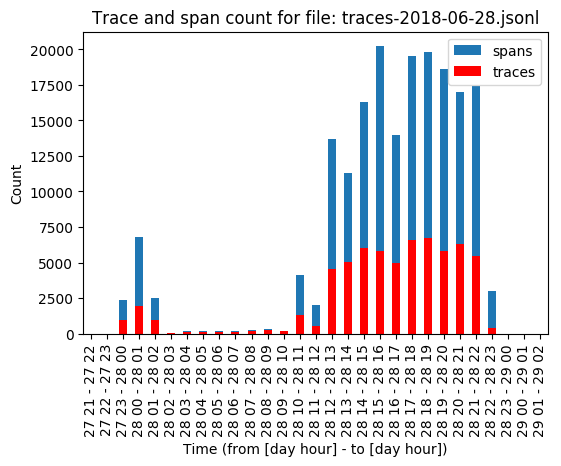
\includegraphics[width=0.88\textwidth]{images/trace_file_count_2018_06_28_chart.png}
    \caption{Trace file count for 2018-06-28.}
    \label{fig:trace_file_count_2018_06_28}
\end{figure}

\begin{figure}[H]
    \centering
    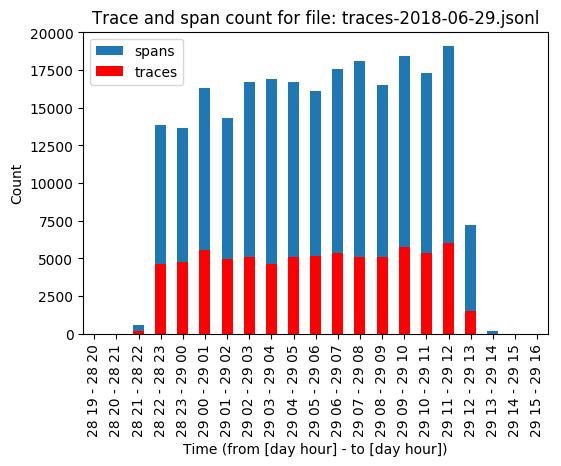
\includegraphics[width=0.88\textwidth]{images/trace_file_count_2018_06_29_chart.png}
    \caption{Trace file count for 2018-06-29.}
    \label{fig:trace_file_count_2018_06_29}
\end{figure}

Figure~\ref{fig:trace_file_count_2018_06_28} presents the counting of traces and spans for the \nth{28} of June, 2018. In this Figure we can spot a ``pit'' in quantity from 2AM to 10AM. No explanation for this was given, however, at this point we assumed that extracting metrics from data in this time interval would produce less points, thus less resolution. This is visible in metrics presented in Figure~\ref{fig:service_calls_samples}, reproduced using \emph{Grafana}. The quantity of data for the rest of the day is somehow inconstant, however, there is no lack of data.

Figure~\ref{fig:trace_file_count_2018_06_29} presents the counting of traces and spans for the \nth{28} of June, 2018. In this Figure there are no ``pits'', and consequently, the quantity of information is more constant throughout time.

To summarise, this system produces an average of 5000 traces an hour and 15000 spans an hour. Also, the quantity of information provided in the second day (\nth{29} of June) is more constant, and therefore, better for analysis, than in the first day (\nth{28} of June). Nevertheless, this data set has sufficient information to study tracing data and develop methods for tracing data, and then, it is a suitable data set for this research project.

Next Chapter, \ref{sec:open_tracing_processor_component}~-~\nameref{sec:open_tracing_processor_component}, covers the explanation and algorithms used over this data set for tracing metrics extraction and quality analysis. Also, some visualizations of metrics extracted from tracing data are provided.

\newpage

\section{OpenTracing Processor Component}
\label{sec:open_tracing_processor_component}

In this Chapter, the implementation for the first component of the proposed solution, \gls{otp}, is presented and explained, hence, functional requirements defined in Table~\ref{sec:functional_requirements}, service dependency graph handling, span trees generation and methods for metrics extraction and storing from tracing data will be covered.

Starting by the first two functional requirements (FR-1 to FR-2). These require communication with distributed tracing tools, to obtain tracing data and to retrieve service dependency graphs. We have decided to use \emph{Zipkin}, as a distributed tracing tool for holding our data set, instead of Jaeger only due to simplicity in setup configuration. To setup this tool a \emph{Docker} container was instantiated in an external server. Communication methods are implemented in \emph{Tracing Collector} component. To feed information to our solution, one can use two ways: collect tracing data from local files, or export them to \emph{Zipkin} and ingest it through \gls{http} requests. This configurations can be changed by editing a configuration file provided with the solution. The configurations to edit are file locations in local machine and \emph{Zipkin} IP (Internet Protocol) address.

After collecting information from one of the two defined sources by \emph{Tracing Collector}, data is passed to \emph{Tracing Processor} which ingests and maps all the information into in memory data structures. Data can be either trace data or service dependency graphs. If it is a graph, it is transferred to \emph{Graph Processor} for process, graph metrics extraction and later storage, otherwise, it is processed in \emph{Tracing Processor} to extract defined metrics from tracing. The algorithm for metrics extraction from tracing and service dependency graphs is presented at a high abstraction level in Algorithm~\ref{alg:metrics_extraction_from_tracing}.

\begin{algorithm}
    \KwData{Trace files/Trace data.}
    \KwResult{Trace metrics written in the time-series database.}
    Connect to Time-Series database\;
    Read time\_resolution, start\_time and end\_time from configuration\;
    Read traces from trace files/trace data\;
    Post traces to Zipkin\;
    Get services from Zipkin\;
    Calculate time\_intervals using start\_time, end\_time and time\_resolution\;
    \While{time\_interval in time\_intervals}{
        Get service\_dependencies from Zipkin\;
        Build service\_dependency\_graph using service\_dependencies\;
        Extract graph\_metrics from service\_dependency\_graph\;
        \While{service in services}{
            Get traces from Zipkin\;
            Map traces in SpanTrees\;
            Extract service\_metrics from SpanTrees\;
        }
        Post graph\_metrics to Time-Series database\;
        Post service\_metrics to Time-Series database\;
    }
    \caption{Algorithm for metrics extraction from tracing.}
    \label{alg:metrics_extraction_from_tracing}
\end{algorithm}

Algorithm~\ref{alg:metrics_extraction_from_tracing} contains some core functionalities implemented in components presented in \gls{otp} solution. This algorithm aims for metrics extraction from tracing data and perform this procedure using two main data structures: service dependency graphs and tracing data mapped into SpanTrees.

\newpage

Service dependency graphs are obtained from \emph{Zipkin} and parsed directly into a \emph{NetworkX} graph structure, presented in component \emph{Graph Processor}. We decided to chose \emph{NetworkX}, a framework for graph processing written in \emph{Python}, due to tooling versatility has it contains a large implementation set of the majority graph algorithms. At this point we preferred this trade-off over processing power and scalability. \emph{Zipkin} provides service dependency graphs through an explicit endpoint -- \emph{/dependencies}, and a start and end timestamps in epoch milliseconds must be passed as parameters. The information comes in \gls{json} format as presented in Listing~\ref{lst:dependencies_zipkin_json}.

\begin{lstlisting}[caption={Zipkin dependencies result schema.},captionpos=b, label={lst:dependencies_zipkin_json}]
    [
        {
            "parent": "string",
            "child": "string",
            "callCount": 0,
            "errorCount": 0
        },
        { /* ... */ }
    ]
\end{lstlisting}

Listing~\ref{lst:dependencies_zipkin_json} shows that dependencies come in an array of \gls{json} objects. Each object contains the information about one relationship between services: parent ``from'', child ``to'' and the number of calls. Therefore, having this information grant the creation of service dependency graph using \emph{NetworkX}. Note that this information assembles a graph containing the information of system services at a specific time interval defined by provided parameters to \emph{Zipkin} \emph{/dependencies} endpoint. After having this information mapped into \emph{NetworkX} graphs in memory, their visual representation are identical to the one demonstrated in Figure~\ref{fig:service_dependency_graph}, presented in Subsection~\ref{subsec:graphs}.

SpanTrees are a representation of a trace in a tree format. Method for their creation from a span list is presented in Algorithm~\ref{alg:spans_to_span_tree}.

\begin{algorithm}
    \KwData{Span list.}
    \KwResult{Spans mapped into SpanTrees.}
    Index spans by ids from span list into SpanIndex\;
    \While{span in span list}{
        Read parentId from span\;
        Index span using parentId into SpanIndex\;
    }
    \caption{Algorithm for SpanTree mapping from spans.}
    \label{alg:spans_to_span_tree}
\end{algorithm}

Algorithm~\ref{alg:spans_to_span_tree} shows that to transform a list of spans (unordered traces) into \emph{SpanTrees}, one must index them by span id an then read every span, indexing the span using their \emph{parentId}. After applying this method, spans will be properly indexed and a list of \emph{SpanTrees} are produced. Also, a SpanTree is a representation of a trace and these structures ease tracing handling due to distinct causal relationships between spans. For example, one can use span trees to map TraceInfos. This data structure was created to hold relevant information from span trees: for example request work-flows. The process involves pinpointing requests between services, presented in spans throughout their causal relationship, and then store request paths through services, generating the corresponding request work-flow. For each span tree, one work-flow is generated, however, from root to leafs, multiple paths are possible. Note that not always do spans contain information to produce the path, and therefore, some request paths are dubious, depending only on the completeness quality of tracing. The method to produce request work-flows is described in Algorithm~\ref{alg:work_flow_type_algorithm}.

\begin{algorithm}
    \KwData{Trace files/Trace data.}
    \KwResult{\gls{csv} with unique work-flow types, their corresponding count and times.}
    Read start\_time and end\_time from configuration\;
    Read SpanList from trace files/trace data within defined time\_frame\;
    \While{have Spans in SpanList}{
        Read Span\;
        Map Span to SpanTrees\;
    }
    \While{have SpanTree in SpanTrees}{
        Read SpanTree\;
        Map SpanTree to TraceInfos\;
        Read TraceInfo\;
        Read work-flows, work-flow count, times, (others) from TraceInfo\;
        Write fields to \gls{csv} files\;
    }
    \caption{Work-flow type algorithm.}
    \label{alg:work_flow_type_algorithm}
\end{algorithm}

The method described in Algorithm~\ref{alg:work_flow_type_algorithm} aims to use tracing to produce span trees, and then generate TraceInfos to retrieve request work-flow paths.

These two data structures, service dependency graphs and span trees, are the foundations to extract metrics from tracing data, satisfy the functional requirements presented in Section~\ref{sec:functional_requirements} and answer the final research questions defined in Section~\ref{sec:research_questions}.

The metrics that \gls{otp} is able to extract from tracing data, for a defined time interval, are the following:

\begin{enumerate}
    \item Number of incoming/outgoing service calls;
    \item Average response time by service;
    \item Service connection, i.e., other services invoking and being invoked by the system, i.e., the service dependency graph variation.
    \item Service degree (in/out/total);
    \item Service \gls{http} status code ratio. (sum of success or failure count over total status code count)
\end{enumerate}

These metrics are all related with time and represent observations of values extracted from tracing data, therefore, as time-series metrics they are stored in a \gls{tsdb}. Explanation of used technology and procedure is provided later on this Section.

Table~\ref{table:research_questions_frs_and_metrics} relates each metric with a functional requirement, and correspondent final research question. Functional requirements are identified by an \emph{id} from Table~\ref{table:functional_requirements_specification}.

\begin{table}[H]
    \caption{Relations between final research questions, functional requirements and metrics.}
    \label{table:research_questions_frs_and_metrics}
    \centering
    \begin{tabularx}{\linewidth} {
        |>{\hsize=0.75\hsize}X|
        >{\hsize=0.60\hsize}X|
        >{\hsize=1.65\hsize}X|}
        \hline
        \textbf{Research} \newline \textbf{Question}
         & \textbf{Functional} \newline \textbf{Requirements}
         & \textbf{Metrics}                                   \\ \hline \hline
        1. Is there any anomalous service?
         & FR-5; \newline
        FR-5; \newline
        FR-6.
         & Number of incoming service calls; \newline
        Number of outgoing service calls; \newline
        Average response time by service.                     \\ \hline
        \textcolor{gray}{2. What is the overall reliability of the service?}
         & FR-7; \newline
        FR-8.
         & No metric extracted; \newline
        Service \gls{http} status code ratio.                 \\ \hline
        \textcolor{gray}{3. Which service consumes more time when considering the entire set of requests?}
         & FR-9; \newline
        FR-10.
         & Service degree; \newline
        Service dependency graph variation.                   \\ \hline
        %4. How can we measure the quality of tracing?
        % & FR-11; \newline
        % FR-12.
        % & 1                                                  \\ \hline
    \end{tabularx}
\end{table}

For Table~\ref{table:research_questions_frs_and_metrics}, only functional requirements from numbers 5 to 10 were considered, due to being the ones related with metrics extraction. As said before, only question number 1 was considered for metrics extraction. The remaining, defined at grey colour, were implemented and \gls{otp} extracts them, however, they were not further analysed in this research. Almost all functional requirements have one metric associated except one, \emph{FR-7}. This functional requirement was implemented, and our solution allows to generate work-flow paths from tracing data, however, no metric was defined. Nevertheless, the implementation of this functionality helped us understanding results for the first final research question -- Method for work-flow generation from tracing data is explained Algorithm~\ref{alg:work_flow_type_algorithm}.

Span trees are a representation of causal relationship between spans. Two types of time based metrics are extracted from span trees: 1. Average response time by service in time; and 2. Service \gls{http} status code ratio in time. To extract the first metric type, \emph{duration} and \emph{annotations/endpoint/serviceName} values presented in spans , when defined, are used to calculate the average response time by service. For each span tree a list of services and their corresponding average times are obtained. After gathering all values from every span tree presented in the defined time-frame, the values are merged and posted to the \gls{tsdb}. The second metric, is extracted through a calculation of status codes ratio by each service. For this, \emph{binaryAnnotations/http.status\_code} and \emph{annotations/endpoint/serviceName} values are used. Also, equally to the previous metric, values are merged and posted to the \gls{tsdb}.

Service dependency graphs are a representation of dependencies of services at a specific time-frame. Three types of time based metrics are extracted from service dependency graphs: 1. Number of incoming/outgoing service calls in time; 2. Entry/exit of services in time (service dependency graph node variation); and 3. Service degree (in/out/total) in time. To extract the first metric type, the values in between (Edges) services (Nodes) are retrieved. These values are dispatched for storage with service name, flow indication (incoming/outgoing), timestamp and number of calls. The second metric type is extracted having two successive graphs and performing their difference. For example, if $Graph A$ has nodes ${A, B, C}$ and $Graph B$, nodes ${A, C, D, E}$, the difference between them will result in two service entries ${D, E}$ and one exit. Last metric type, service degree, is extracted by retrieving the number of connections from each service. For example, consider that $Graph C$ has a service $A$ connected from itself to services ${B, C, D}$. In this graph, service $A$ has an out degree of three and an in degree of zero. The remaining services have an out degree of zero and an in degree of one. Methods to extract these metrics are implemented in \emph{Graph Processor} and resource to \emph{NetworkX} to handle graph structures. All these metrics are then posted to the \gls{tsdb}.

At this point, our solution is able to retrieve and store time-series metrics from tracing data. For the \gls{tsdb}, we have decided to use \emph{OpenTSDB}, due to technical restrictions imposed in Section~\ref{sec:technical_restrictions}. There was a client implementation for usage in \emph{Python}, however, the support was not good due to lack of updates and clear documentation. For this reason, we decided to implement our own \emph{OpenTSDB} client in \emph{Python} using their \gls{api} specification, -- \emph{Metrics Repository} component. Later, when all implementation from tracing collection through trace metrics storage in the \gls{tsdb}, we used a browser metrics visualizer. To do this, a \emph{Docker} container with \emph{Grafana}, a data visualization tool capable of rendering time-series metrics in charts and present them in dashboards. The decision to use this tool, was due to easy to setup and integrated compatibility with our \gls{tsdb}. We just needed to create a container and, through a url configuration in \emph{Grafana}, we established a link to the \gls{tsdb}.

Figures~\ref{fig:service_dependency_variation}, ~\ref{fig:service_calls_samples},~\ref{fig:service_avg_response_time_samples}, and~\ref{fig:service_status_code_ratio_samples}, contain sample representations of extracted time-series metrics stored in our \gls{tsdb}.

\begin{figure}[H]
    \centering
    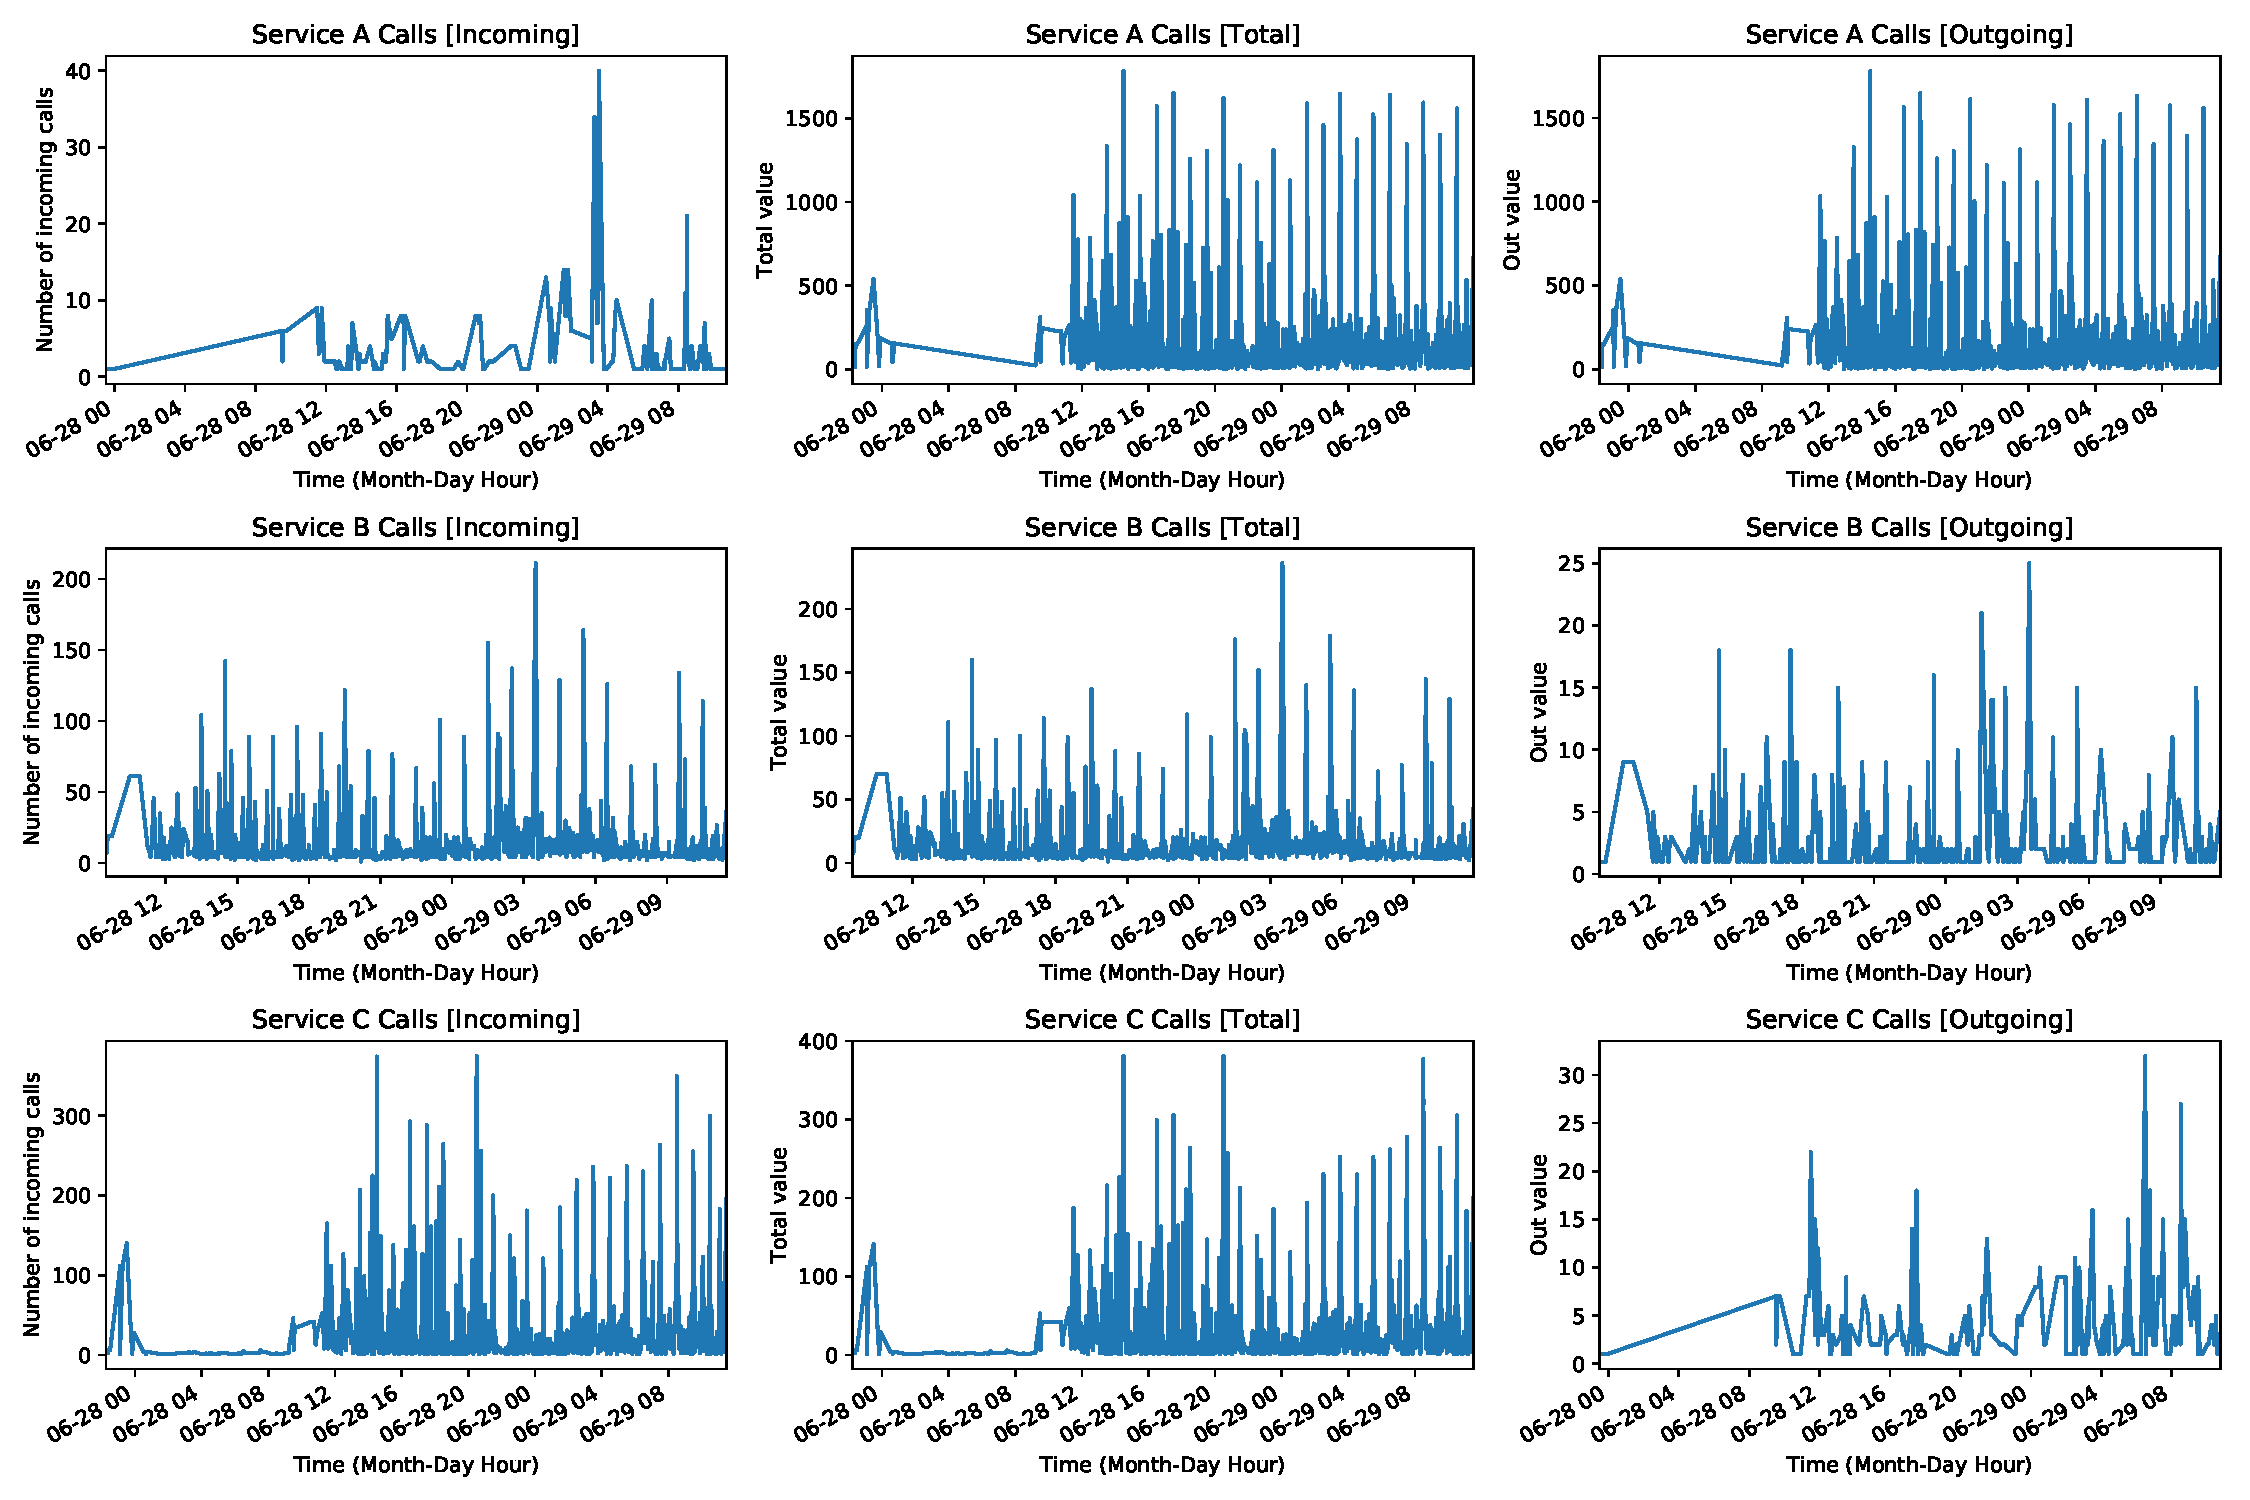
\includegraphics[width=1.00\textwidth]{images/service_calls.pdf}
    \caption{Service calls samples.}
    \label{fig:service_calls_samples}
\end{figure}

\begin{figure}[H]
    \centering
    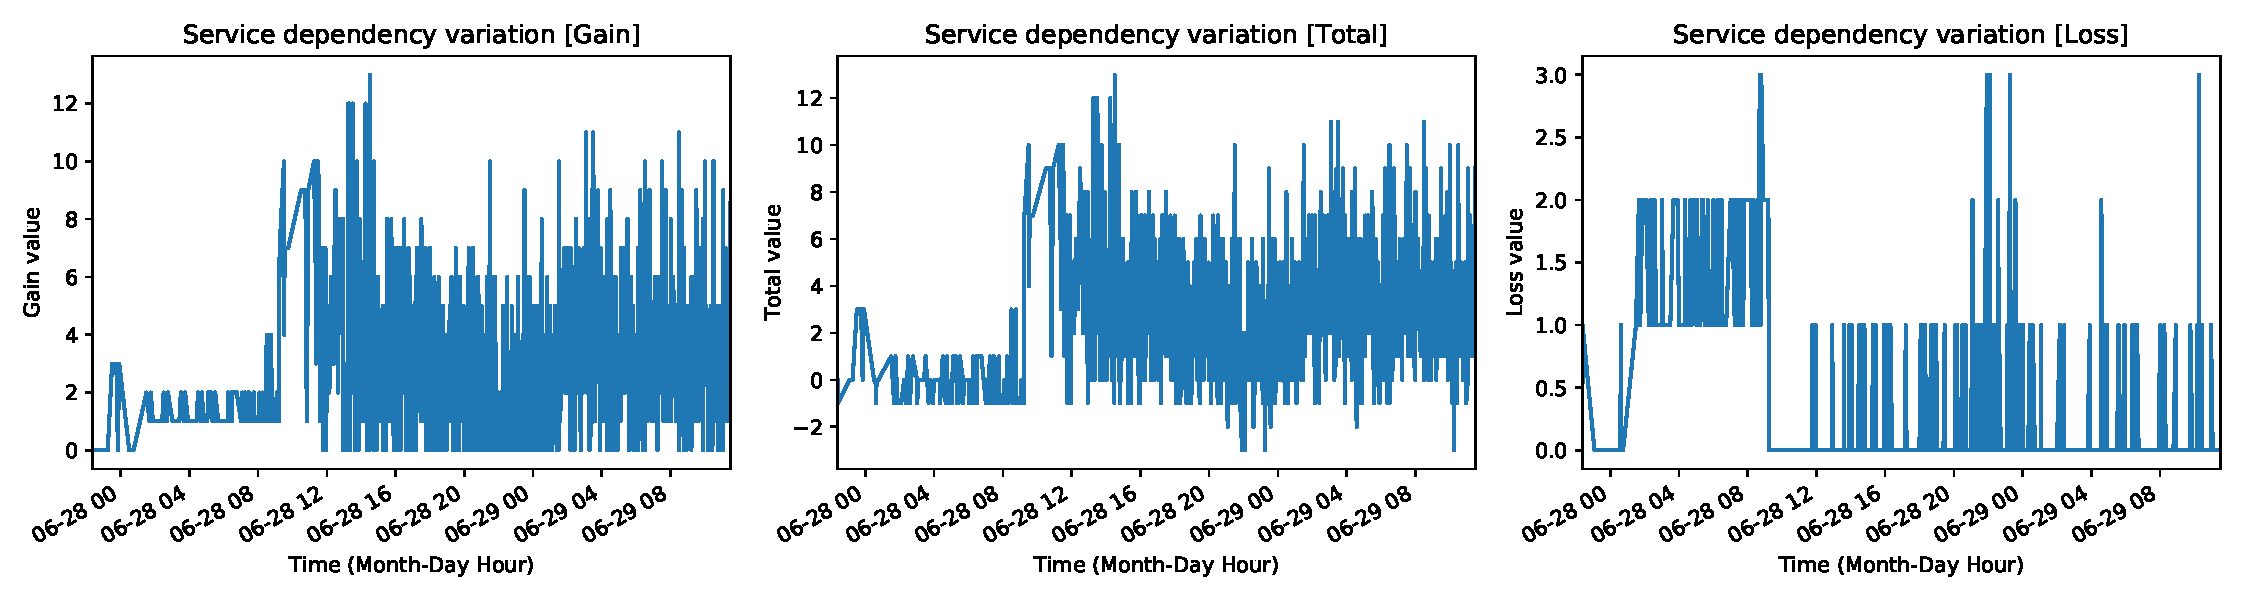
\includegraphics[width=1.00\textwidth]{images/service_dependency_variation.pdf}
    \caption{Service dependency variation samples.}
    \label{fig:service_dependency_variation}
\end{figure}

\begin{figure}[H]
    \centering
    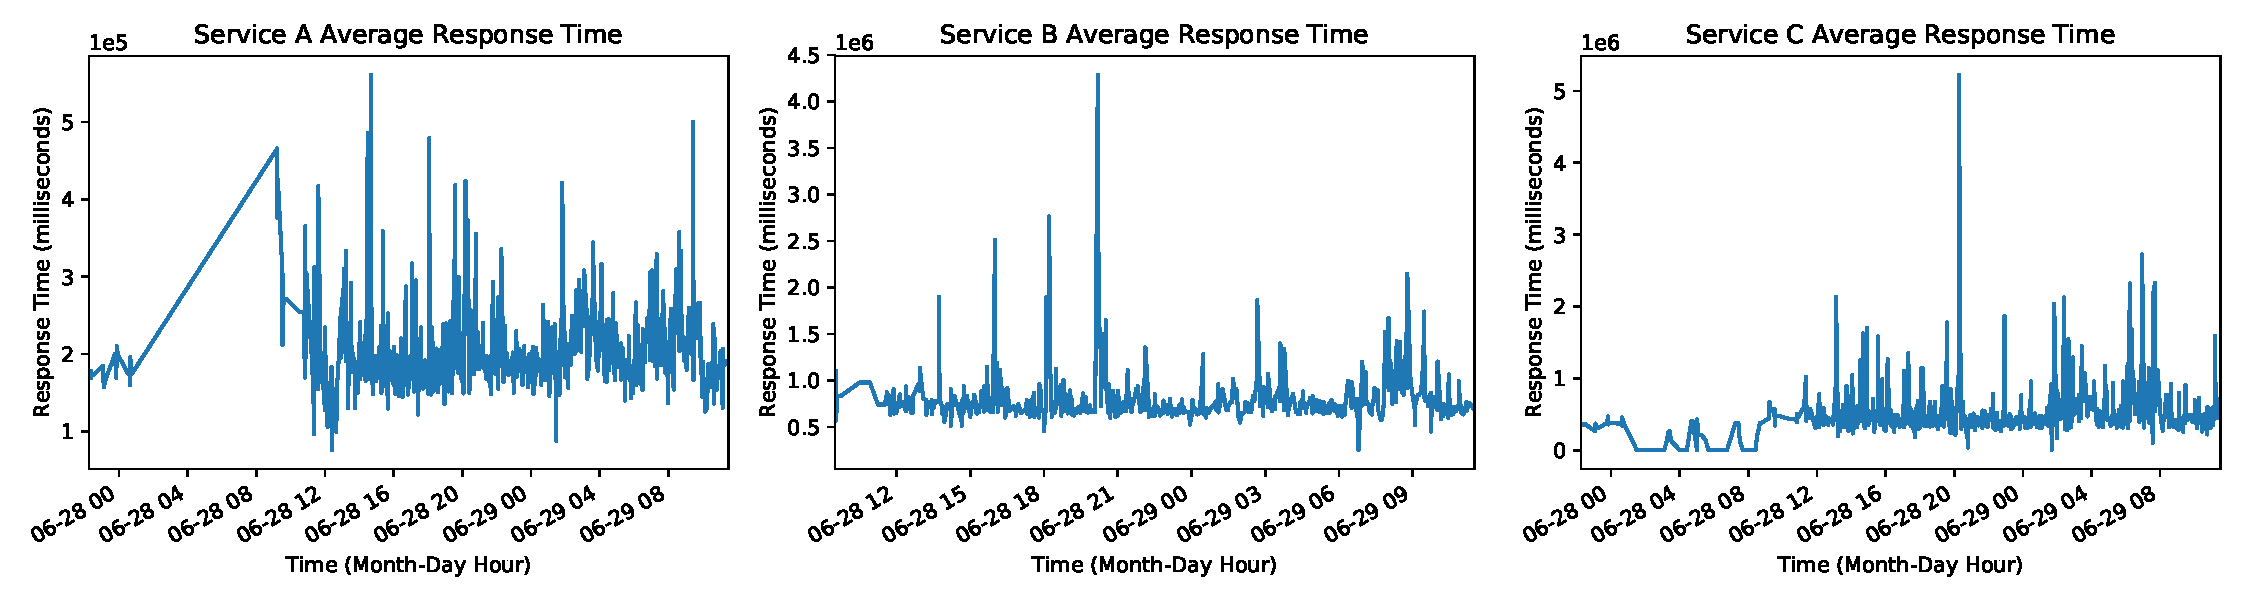
\includegraphics[width=1.00\textwidth]{images/service_avg_response_time.pdf}
    \caption{Service average response time samples.}
    \label{fig:service_avg_response_time_samples}
\end{figure}

%\begin{figure}[H]
%    \centering
%    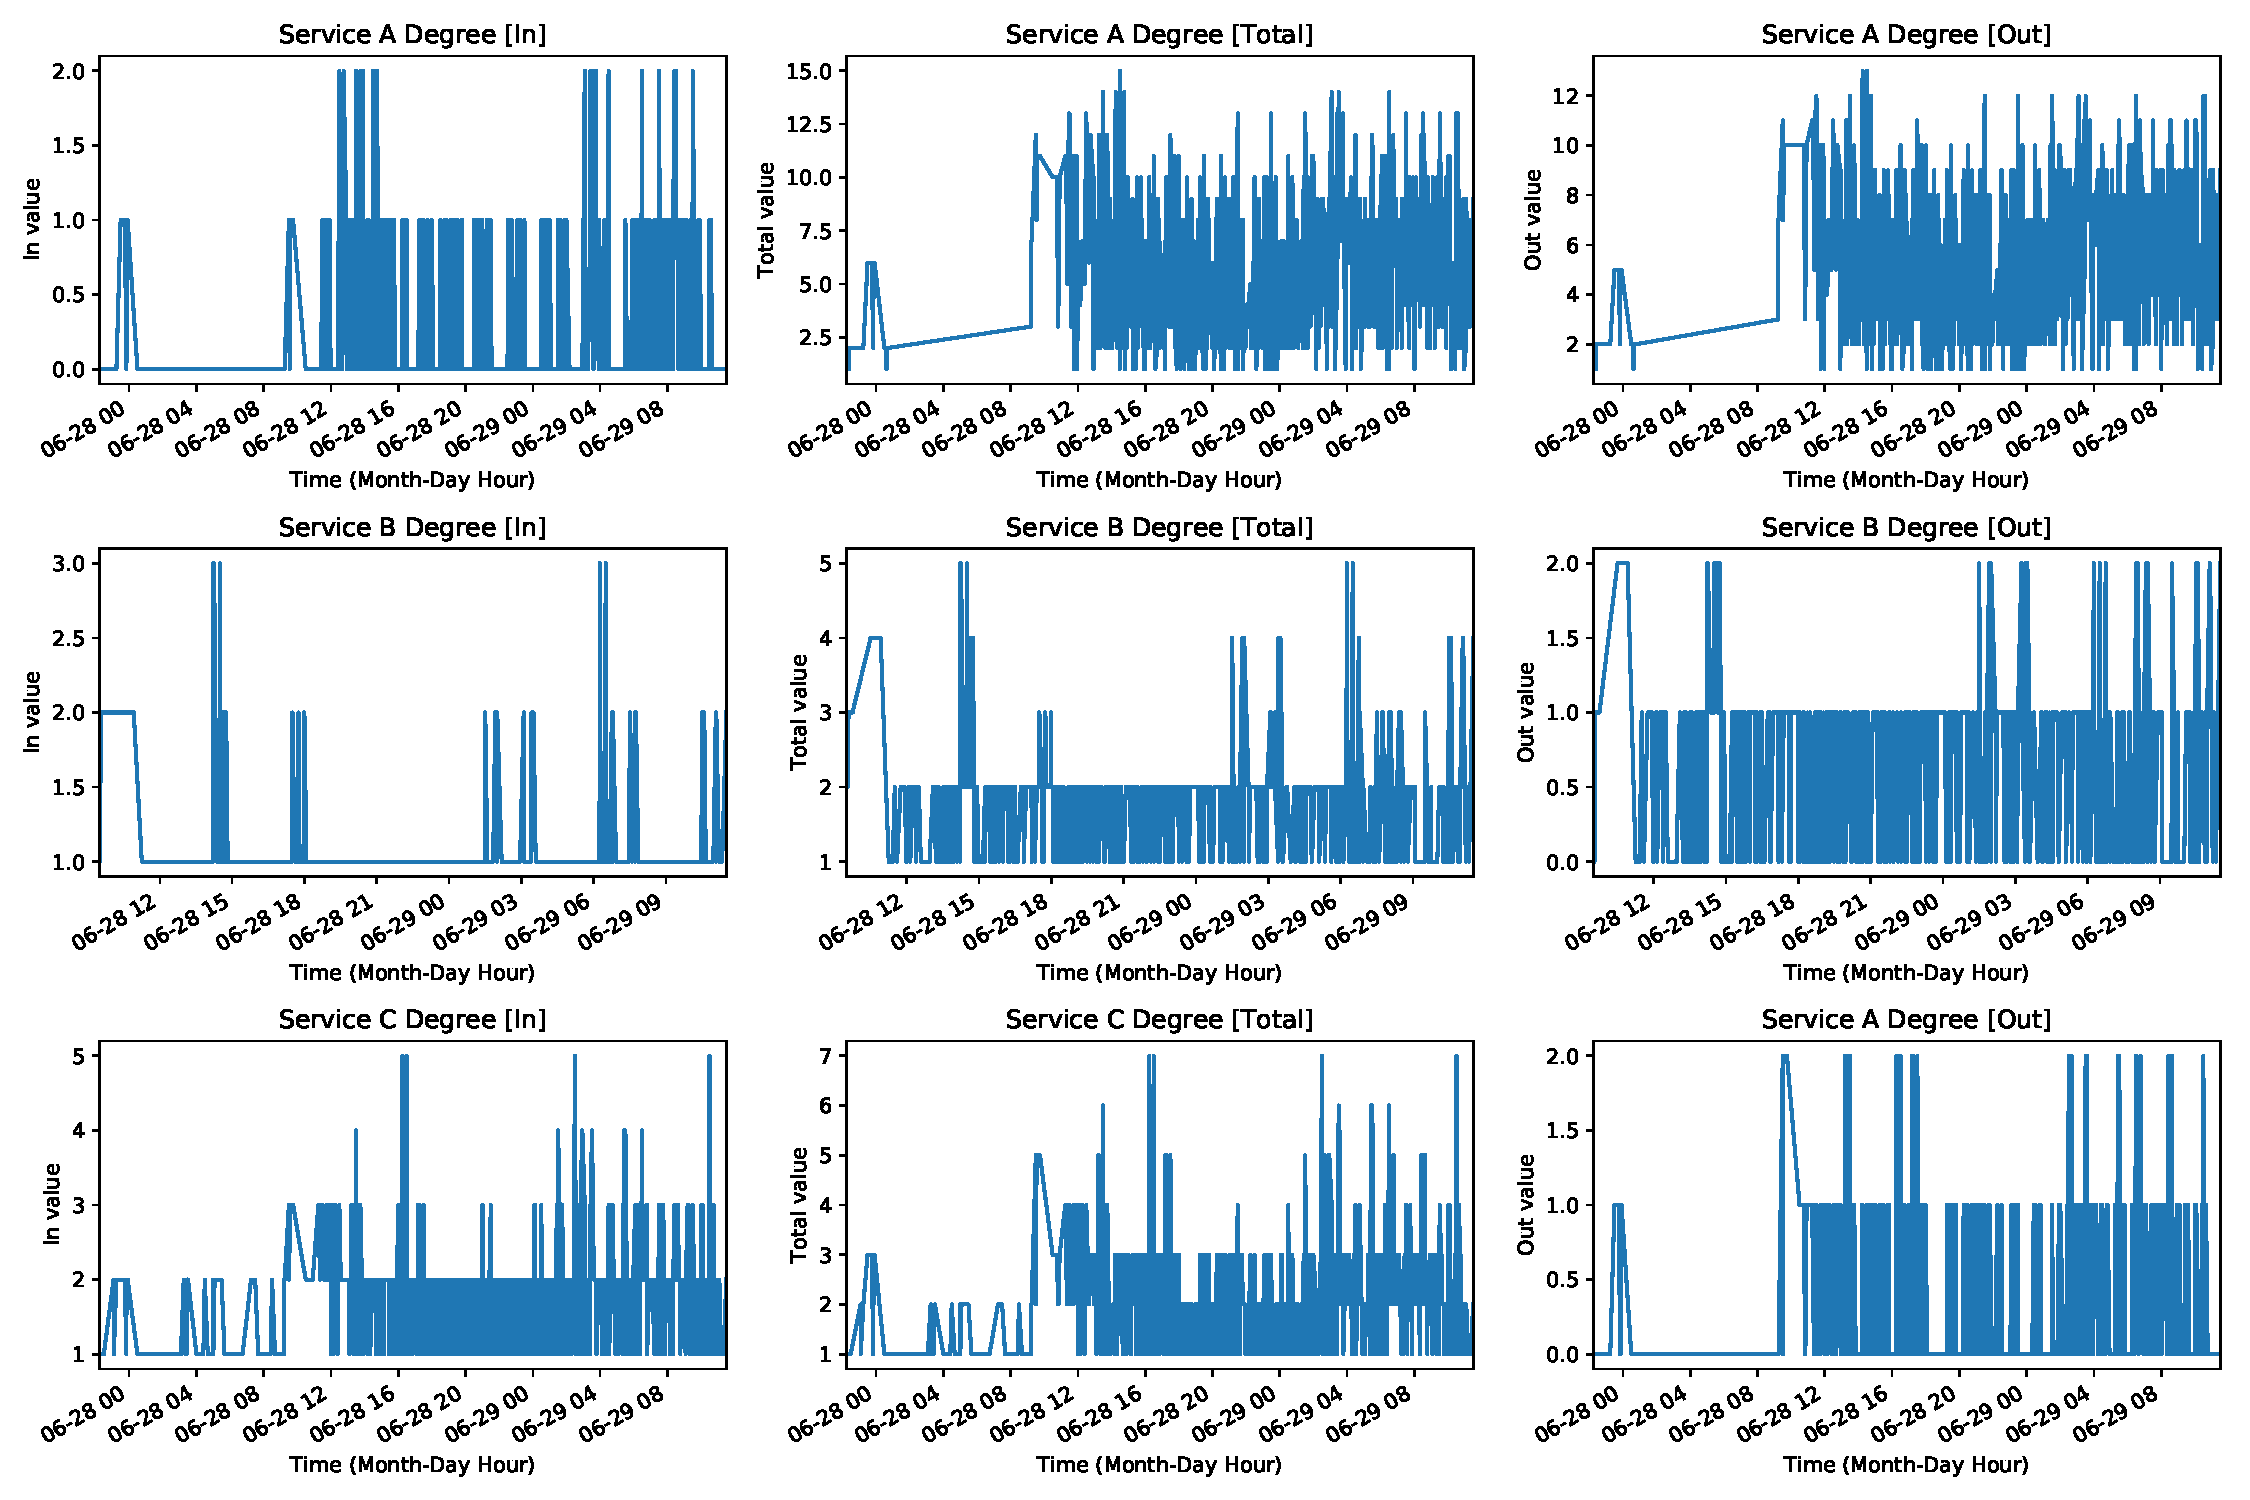
\includegraphics[width=1.00\textwidth]{images/service_degrees.pdf}
%    \caption{Service degree samples.}
%    \label{fig:service_degree_samples}
%\end{figure}

\begin{figure}[H]
    \centering
    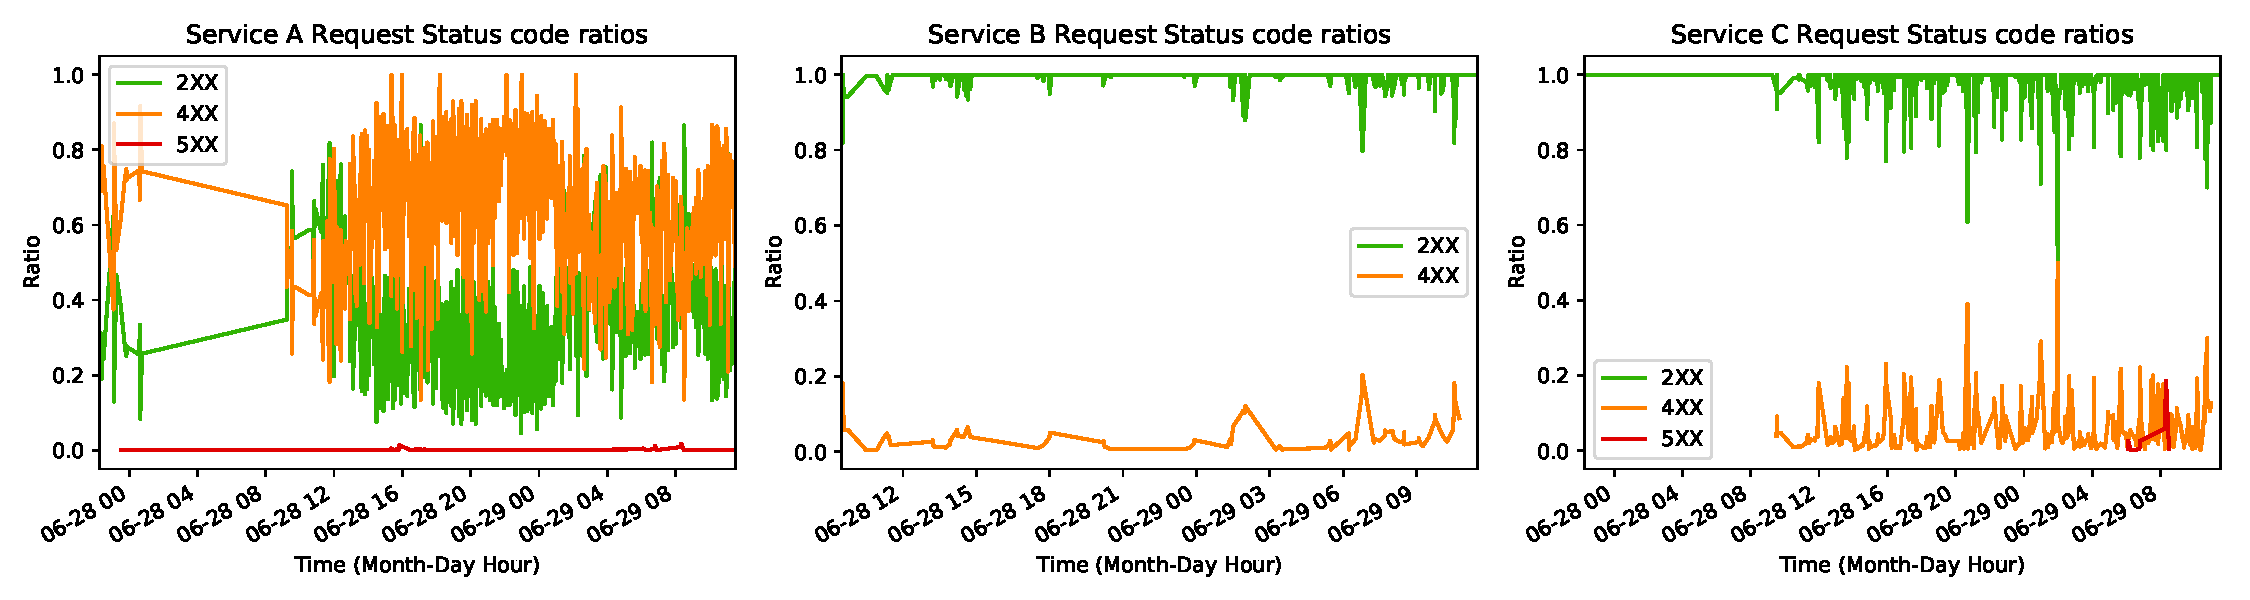
\includegraphics[width=1.00\textwidth]{images/service_status_code_ratio.pdf}
    \caption{Service status code ratio samples.}
    \label{fig:service_status_code_ratio_samples}
\end{figure}

Figure~\ref{fig:service_calls_samples} represent samples about the number of service request calls metric. In this Figure, we have 9 plots, three in each row. Each row represents three variations (incoming, outgoing and total) of this metric for one service. In this metric we can clearly see the lack of information presented in tracing for the beginning of the first day.

Figure~\ref{fig:service_dependency_variation} contain samples about service dependency variation, one for each metric (gain, loss and total). Total are the result of $gain - loss$. Gain stands for the number of new service entries in system, and loss, represent the number of service exits in system.

Last Figure,~\ref{fig:service_status_code_ratio_samples}, shows the gathering of status code ratio samples for three distinct services. The ratio varies from 0.0 to 1.0, and represent the proportion of status code groups (2xx -- Success, 4xx -- Client error and 5xx -- Other errors).

Also, service dependency graphs are stored for further access after being processed by \emph{Graph Processor} component. We have decided to use \emph{ArangoDB} as our \gls{gdb}. This decision was based in the ``Multi data-type support'' provided by this database, allowing us to extend our graph structures to whatever we wanted, enhancing our graph storage possibilities and relieving the implementation from parsing data-types. This database has a \emph{Python} client, \emph{pyArango}~\cite{pyarango}, which revealed lack of features, leading to propositions for functionality creation and issue declarations in GitHub. However, the answers were not pleasant due to lack of support and people to maintain the project~\cite{arango_issues}. This have lead to some difficulties when implementing \emph{Graphs Repository} component in \gls{otp}. Difficulties from storing graphs with custom names to custom graph retrieval were felted. The solution was to fork the project, perform changes and use our custom \emph{pyArango} client. This changes were committed for review to the original project. Mitigating this kind of problems in advance, was impossible because they were only perceived when using the client.

%Also, service dependency graphs are processed and stored in a \gls{gdb}, however, they do not have further use for this research. The decision to keep them and store them, eases their retrieval and further usage on upcoming projects.

After presenting the first component, \gls{otp}, from our proposed solution, next Section~\ref{sec:data_analysis_component}~-~\nameref{sec:data_analysis_component} covers the implementation of the second component presented in our solution.

\section{Data Analysis Component}
\label{sec:data_analysis_component}

In this Section, the implementation of the second component presented in our proposed solution, ``Data Analysis'' component, is presented and expected outcomes from each analysis are discussed.

``Data Analysis'' component has the main objective of detecting anomalies, presented in services, using time-series metrics extracted from tracing data using the component presented in previous Section and perform tracing quality analysis.

In our implementation, this component is detached from the remaining components, however, in architectural terms we have decided to place it has being part of the overall solution. This is because there is nothing preventing total integration with other components presented in the solution. The reason to implement these methods detached from the remaining, was to ease our research path and increase flexibility. This means that, to ease our data exploration, implement these methods in Notebooks detached from the overall components, allowed us to change code effortlessly and conceded focus on methods development. Jupyter Notebook~\cite{jupyter_notebooks} was the notebook chosen for method implementation, hence, one server was created to hold our implementations in notebooks.

In this case, extracted time-series data belong to unlabelled data group. Data can belong to unlabelled or labelled groups. Unlabelled data are information sampled from of natural, or human-created artefacts, that one can obtain from observing and record values. In this group, there is no ``explanation'' for each piece of data, as it just contains the data, and nothing else. Labelled data typically takes a set of unlabelled data and augments each piece of data with some sort of meaningful ``tag'', ``label'', or ``class'' that is somehow informative or desirable to know. For example, for this solution, having labelled data would help in identifying anomalies presented in our data set. However, only unlabelled data was provided, and therefore, we needed to work with unlabelled data and perform anomaly detection with it~\cite{Kothari}.

So, the approach was to use processed data produced from \gls{otp}, and perform the analysis using ``Data Analysis'' component to point out service problems and perform tracing quality analysis, as defined in Figure~\ref{fig:proposed_approach}, to answer questions defined in Chapter~\ref{chap:research_objectives_and_approach}:

\begin{enumerate}
    \item Is there any anomalous behaviour in the system? (If yes, where?);
    \item How can we measure the quality of tracing?
\end{enumerate}

To answer the first question, using our proposed solution, one must use metrics extracted from tracing data, namely the number of incoming / outgoing requests and the average response time for each service. These metrics are time-series metrics, and therefore, anomaly detection using unsupervised learning algorithms are the way to do it~\cite{Brillinger2006}. Metrics were obtained using methods defined in our \emph{OpenTSDB} client, implemented in \emph{Metrics Repository} component.

After extracting these metrics, they are allocated in a data structure called \emph{dataframe} from \emph{Pandas}, an open source library that provides high-performance, easy-to-use data structures and data analysis tools. This library was chosen due to being one of the most used and popular for this purpose~\cite{pandas} -- data science and data analysis. A \emph{Dataframe} is a two-dimensional size-mutable, potentially heterogeneous tabular data structure with labelled axes (rows and columns).  In these data structures, values from time-series metrics were stored in columns: \emph{timestamp} (index), \emph{datetime}, \emph{number\_of\_incoming\_requests}, \emph{number\_of\_outgoing\_requests} and \emph{average\_response\_time}. In the end, a list of \emph{dataframes} are created, one \emph{dataframe} for each service.

Before performing an analysis to detect if there are outliers presented in our data, the information must be checked and tested to verify if data have missing values. This is done because metrics are extracted from multiple sources and thus generates missing values. For example, we may have missing information for one of the three features in a row of one \emph{dataframe}. Missing values are a pain in data analysis and are represented by \emph{NaN} in \emph{dataframes}, and for this reason,one can not apply anomaly detection algorithms over data with missing values. To fulfil missing information there are two approaches:

\begin{enumerate}
    \item Remove rows with missing values, which degrades the overall data and may result in insufficient data;
    \item Impute missing values, however, it may be dangerous because it introduces "wrong" observations.
\end{enumerate}

We decided to impute missing values because there were too keep information quantity. However, there are multiple ways for imputation of missing values into time-series data, depending on factors of trend and seasonality. Trending is the increasing or decreasing value in the series, and seasonality is the repeating short-term cycle in the series~\cite{Brillinger2006}. Figure~\ref{fig:methods_to_fulfil_time_series_data} shows the path to chose the correct method to fulfil information in time-series data.

\begin{figure}
    \centering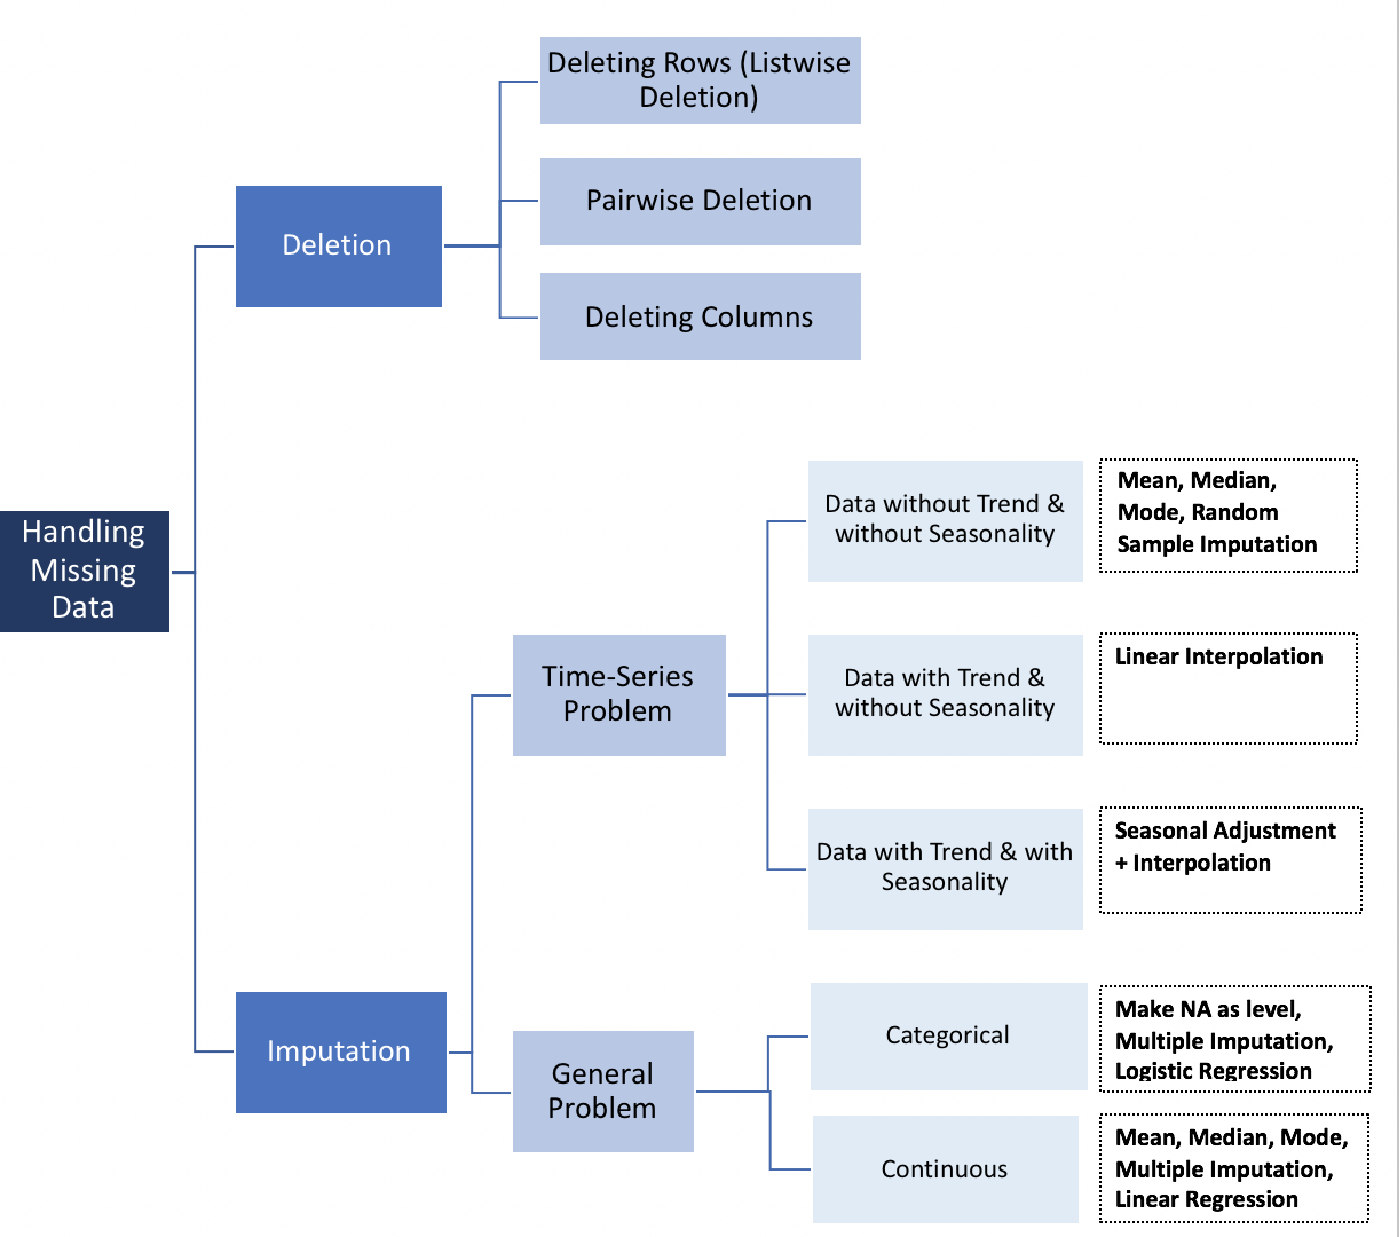
\includegraphics[width=0.8\linewidth]{images/methods_to_fulfil_time_series_data.pdf}
    \caption{Methods to handle missing data~\cite{Swalin2019}.}
    \label{fig:methods_to_fulfil_time_series_data}
\end{figure}

So, before applying the method, our component tests the data to chose the correct method to fulfil data. Figure~\ref{fig:trend_seasonality_results} contains trend and seasonality sample tests performed over our data.

\begin{figure}
    \centering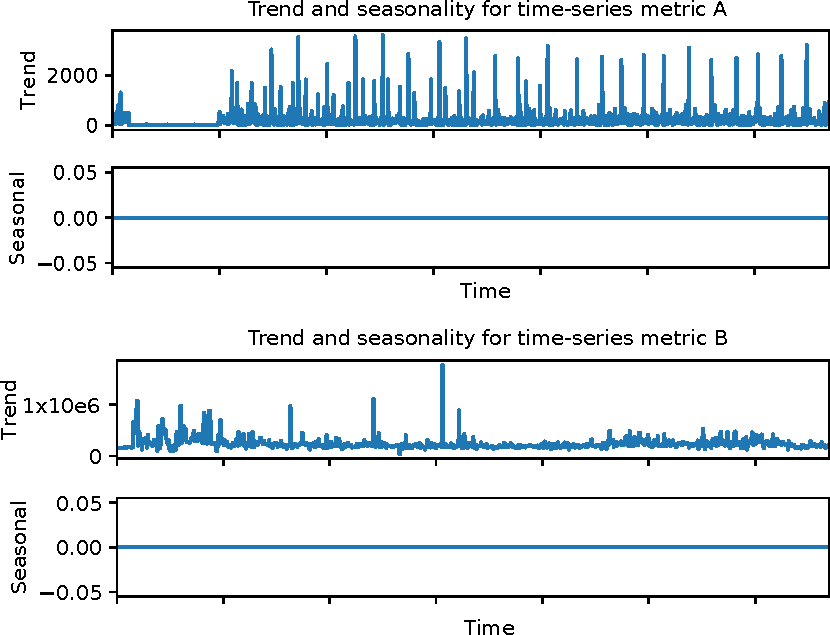
\includegraphics[width=0.8\linewidth]{images/trend_seasonality_results.pdf}
    \caption{Trend and seasonality results.}
    \label{fig:trend_seasonality_results}
\end{figure}

Figure~\ref{fig:trend_seasonality_results} shows that there are clearly trends in our data, however, no seasonality was detected. For this reason, the selected method to fulfil data presented in \emph{dataframes} is Linear Interpolation -- Figure~\ref{fig:methods_to_fulfil_time_series_data}.

These \emph{dataframes} are then processed by an unsupervised learning algorithm to detect if there are outliers. For the unsupervised learning algorithm there were: Isolation Forests and OneClassSVM~\cite{Zhou2017}. The first one uses binary decision trees to isolate data points and identify outliers presented in the data set, the second one, generates density areas using max-margin methods, i.e. they do not model a probability distribution, hence the idea is to find a function that is positive for regions with high density of points, and negative for small densities, identifying outliers presented in data. Figure~\ref{fig:isolation_forests_and_oneclasssvm_comparison} displays the error comparison of these two methods.

\begin{figure}[H]
    \centering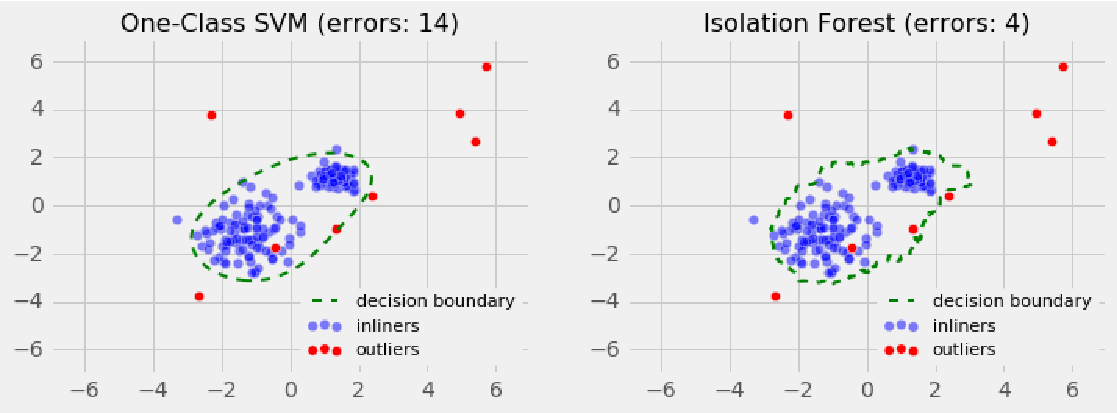
\includegraphics[width=0.8\linewidth]{images/isolation_forests_and_oneclasssvm_comparison.pdf}
    \caption{Isolation Forests and OneClassSVM methods comparison~\cite{isolation_forests_and_oneclasssvm_comparison}.}
    \label{fig:isolation_forests_and_oneclasssvm_comparison}
\end{figure}

From Figure~\ref{fig:isolation_forests_and_oneclasssvm_comparison}, isolation forests prove to be a better method for outlier detection because, from this test, it resulted in fewer errors as it did not construct a parametric representation of the search space. For this reason, we decided to use Isolation Forests, to detect and identify outliers presented in time-series metrics extracted from tracing data. To implement Isolation Forests method we used Scikit-Learn, a library full of simple and efficient tools for data mining, data analysis and machine learning. All configurations used from this library to implement Isolation Forests were setted to default. Therefore, Algorithm~\ref{alg:anomaly_detection} presents the whole process to identify anomalous services presented in the system.

\begin{algorithm}
    \KwData{Processed data from tracing using \gls{otp}.}
    \KwResult{Report, in \gls{csv} file, containing identified anomalous services and correspondent times.}
    Read start\_timestamp, end\_timestamp, db\_settings from configuration\;
    Connect to \gls{tsdb}\;
    Retrieve metrics from \gls{tsdb} using database connection, start\_timestamp and end\_timestamp\;
    Create dataframes with metrics data\;
    Perform data imputation over dataframes\;
    Feed Isolation Forests with metric columns from dataframes\;
    Fire Isolation Forests method (Adds new column ``anomaly'' with -1 ``Anomalous'' or 1 ``Non-anomalous'')\;
    Filter ``anomaly'' column with -1 values from dataframes into anomalous\_dataframes\;
    Write report with anomalous service names and times from anomalous\_dataframes data\;
    \caption{Anomalous service detection algorithm.}
    \label{alg:anomaly_detection}
\end{algorithm}

Algorithm~\ref{alg:anomaly_detection} contains all the process explained above. The final outcome from this algorithm is a report containing all anomalous services and correspondent times identified. Also, later we decided to study further the pattern observed in anomalous regions. For this, the approach was to use the algorithm defined in ~\ref{alg:work_flow_type_algorithm} to analyse what happens to work-flows in ``anomalous'' and ``non-anomalous'' regions.

To answer the second question, it requires to perform a structural and time coverage analysis. For the first analysis, the approach is to define a specification schema based on \emph{OpenTracing} open source specification. This schema aims to test span structures in order to detect structural problems present in spans, e.g., missed fields, wrong data types, typos presented in structure. The method implemented is presented in Algorithm~\ref{alg:span_structure_analysis_algorithm}.

\begin{algorithm}
    \KwData{Trace files/Trace data.}
    \KwResult{\gls{csv} file reporting span structure analysis.}
    Read specification from open\_tracing\_specification\_schema.json\;
    \While{not end of tracing}{
        Read Span\;
        Check Span against specification\;
    }
    Write results from ``Check'' to \gls{csv} file\;
    \caption{Span structure analysis algorithm.}
    \label{alg:span_structure_analysis_algorithm}
\end{algorithm}

As we can see in Algorithm~\ref{alg:span_structure_analysis_algorithm}, our method aims to produce a report containing the results of span structural analysis. To do this, first it needs to read the \emph{OpenTracing} specification schema. This schema is written in a \gls{json} file, where the fields are annotated with tags: \emph{required}, \emph{data-type: <string, int, other>} and others. \gls{json} Schema~\cite{json_schema_library} was the library used to verify if each span complies with the specification. For the second analysis, the approach is to use spans presented in trace data to analyse the coverage of each trace. Figure~\ref{fig:trace_time_coverage} presents an example for time coverage in a trace.

\begin{figure}[H]
    \centering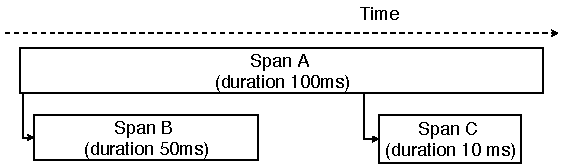
\includegraphics[width=0.8\linewidth]{images/trace_time_coverage_example.pdf}
    \caption{Trace time coverage example.}
    \label{fig:trace_time_coverage}
\end{figure}

Figure~\ref{fig:trace_time_coverage} gives us an example in which we have a trace with a root span of 100 milliseconds of duration, and this root span has two children spans, one with $50ms$, the other one with $10ms$, the entire trace has a coverage of $(50+10)/100=60\%$. This method is applied to every trace, and the results are the stored in a \gls{csv} file to be plotted for visualisation. In this case we apply it and split the results by service, with the objective of perceive the time coverability of tracing in each service. The method is presented in Algorithm~\ref{alg:trace_coverability_analysis}.

\begin{algorithm}
    \KwData{Trace files/Trace data.}
    \KwResult{\gls{csv} file for each service reporting the coverability analysis.}
    Read start\_time and end\_time from configuration\;
    Get services from Zipkin\;
    \While{service in services}{
        Get traces from Zipkin using service, start\_time and end\_time\;
        Map traces in SpanTrees\;
        Calculate trace\_coverability using SpanTrees\;
        Write trace\_coverability to \gls{csv} file\;
    }
    \caption{Trace coverability analysis algorithm.}
    \label{alg:trace_coverability_analysis}
\end{algorithm}

Algorithm~\ref{alg:trace_coverability_analysis} uses \emph{SpanTrees} to calculate \emph{trace\_coverability}, this is due to causal relationships presented in these trees. As explained above, through Figure~\ref{fig:trace_time_coverage}, one must have a trace mounted in span relationships (span trees), to know when a span is child of another, and be able to calculate the coverability presented in a trace. This method performs this calculation for every service and, in the end, stores information about trace coverability into a \gls{csv} file. This file is later used to produce plots about the service trace coverability. What is expected from this method is that we achieve a plotting, where every service has a counting of traces that cover a certain amount of time.

\todo{TALK A LITTLE BIT MORE???}

To summarise, this tools gathers processed data and time-series data from our \gls{tsdb}, extracted using \gls{otp} from original trace information. Then it perform data imputation to solve missing values problems, analyses resulting data using Isolation Forests, an unsupervised multiple feature machine learning algorithm, to identify outliers presented in our extracted metrics, and therefore, detect anomalies presented in services, identifying their occurrences in time. Also, this tools uses tracing to perform an analysis about the structure of spans presented in tracing, and uses processed data from \gls{otp}, to perform an analysis of time coverage provided by tracing data.

Next Chapter~\ref{chap:results_analysis_and_limitations}, we will cover results obtained by this component, discuss these results and present \emph{OpenTracing} data limitations.

\checkoddpage
\ifthenelse{\boolean{oddpage}}
{ % Odd page
    \newpage
    \blankpage}
{ % Even page
}